%%%%%%%% ICML 2026 Mechanistic Interpretability Workshop %%%%%%%%
% Format: ICML 2024 style (semantically equivalent to ICML 2026)
% Submission: double-blind (no \accepted option used).
\documentclass{article}

\usepackage[T1]{fontenc}
\usepackage{microtype}
\usepackage{graphicx}
\usepackage{booktabs}
\usepackage{amsmath,amssymb,amsthm,mathtools}
\usepackage{xspace}
\usepackage{xcolor}
\usepackage{enumitem}
\usepackage{tikz}
\usepackage{pgfplots}
\pgfplotsset{compat=1.18}
\usetikzlibrary{positioning,arrows.meta,shapes.geometric,fit,backgrounds}
\usepackage{hyperref}
\usepackage{icml2024}

% Macros
\newcommand{\maxtoki}{MaxToki-217M\xspace}
\newcommand{\maxtokibig}{MaxToki-1B\xspace}
\newcommand{\geneformer}{Geneformer V2-316M\xspace}
\newcommand{\scfm}{SCFM\xspace}

\icmltitlerunning{Agent-Driven Mech-Interp on \maxtoki{}}

\begin{document}

\twocolumn[
\icmltitle{An Agent-Driven Pipeline for Mechanistic Interpretability\\
of Single-Cell Foundation Models:\\
Findings on \maxtoki{} and a Reusable Audit Framework}

\icmlsetsymbol{equal}{*}
\begin{icmlauthorlist}
\icmlauthor{Anonymous Authors}{anon}
\end{icmlauthorlist}
\icmlaffiliation{anon}{Anonymized for double-blind review}
\icmlcorrespondingauthor{Anonymous Authors}{anonymous@example.com}

\icmlkeywords{mechanistic interpretability, single-cell foundation models, sparse autoencoders, autonomous agents}

\vskip 0.3in
]

\printAffiliationsAndNotice{}

\begin{abstract}
We deploy an agent-driven mechanistic-interpretability pipeline against
\maxtoki{}~\citep{maxtoki2026}, a recently released trajectory-aware
single-cell foundation model, with eight pipelines executed end-to-end
by Claude agents under $\sim$15 hours of human supervision. The model
encodes cell \emph{identity geometry} but not directed \emph{regulatory
mechanism}: five methodologically distinct probes converge on a
negative for fine-grained TF$\to$target logic, while a hematopoietic
developmental manifold is externally generalizable and compressible
$2{,}400\times$ to a 7.7~KB sparse operator, and activation steering
at L0/L3/L9/L11 is causally effective with a non-monotonic mid-layer
basin at L6. An audit-driven re-test inverts the original ``0\% TF
specificity'' headline at strict ChIP-seq threshold
($p_{\text{null}}{=}0.030$, post-hoc, $n{=}1$, awaits replication).
We contribute (i) the agent-driven pipeline architecture, (ii) a
reusable 10-pattern audit framework that detected three load-bearing
flaws in our own runs, and (iii) the deployment study; all pipeline
execution and audit were performed by AI agents.
\end{abstract}

\section{Introduction}

Single-cell foundation models (\scfm{}s) such as
scGPT~\citep{cui2024scgpt}, Geneformer~\citep{theodoris2023geneformer},
scFoundation~\citep{hao2024scfoundation}, and the recently released
\maxtoki{}~\citep{maxtoki2026} are increasingly used for in-silico
perturbation~\citep{lotfollahi2019scgen,roohani2024gears}, GRN
inference, cell-type identification, and drug-target prioritization.
Whether they actually \emph{encode} the biology that downstream uses
rely on, versus merely re-organizing co-expression structure, is an
open question~\citep{kedzierska2023assessing,liu2023evaluating,wenteler2024perteval}.
Mechanistic interpretability addresses this directly: hypothesis-driven,
intervention-supported analysis of what features inside a trained
model represent and how they
compose~\citep{bricken2023monosemanticity,conmy2023acdc,wang2023ioi,sharkey2025open}.
A methodologically defensible mech-interp audit of one \scfm{} can
take many person-months.

Recent autonomous-agent systems --- the AI
Scientist~\citep{lu2024aiscientist}, Coscientist for autonomous
chemistry~\citep{boiko2023autonomous},
ChemCrow~\citep{mbran2024chemcrow}, ML-engineering benchmarks like
MLE-bench~\citep{chan2024mlebench}, and SWE-agent for software
engineering~\citep{yang2024sweagent} --- show that LLM agents can carry
out multi-step research with moderate-to-high autonomy. We
investigate whether mech-interp on \scfm{}s can be largely automated.
Eight mech-interp pipelines, originally developed in the authors'
prior work on scGPT and
Geneformer~\citep{anon2026attention,anon2026spectral,anon2026topology,anon2026sae,anon2026circuits,anon2026manifold,anon2026exhaustive},
are pre-authored as markdown executable specifications and executed
end-to-end against \maxtoki{} by Claude Opus~4.7 agents under
high-level human direction.

\paragraph{Contributions.} (1)~An \emph{agent-executable pipeline
architecture} in which markdown specifications act as executable
contracts for LLM-based research agents. (2)~A \emph{recurring-issue
audit framework} of ten reviewer-derived patterns codified as
agent-applicable diagnostics; in this study the audit shifted three
load-bearing verdicts. (3)~A deployment study yielding six
interrelated findings on \maxtoki{} that jointly characterize the
model as encoding cell-identity geometry but not regulatory mechanism.

\section{Related Work}

\paragraph{\scfm{} mech-interp.} Prior work on scGPT and Geneformer
established the standard catalogue: per-layer attention extraction
with TRRUST/STRING comparison~\citep{anon2026attention},
residual-stream SVD geometry mapping subcellular localization and PPI
networks~\citep{anon2026spectral}, topological hypothesis
screening with hierarchical null
models~\citep{anon2026topology}, SAE atlases of the residual
stream and causal circuit
tracing~\citep{anon2026sae,anon2026circuits}, and manifold
discovery with extraction and
compactification~\citep{anon2026manifold}. Convergent
observation across this lineage: \scfm{}s reorganize co-expression
structure and encode coarse cell-type identity but encode fine-grained
regulatory logic
poorly~\citep{kedzierska2023assessing,liu2023evaluating,wenteler2024perteval}.

\paragraph{Mech-interp foundations.} Sparse
autoencoders~\citep{bricken2023monosemanticity,cunningham2023sparse,templeton2024scaling,gao2024scalingsae}
and activation patching / circuit
tracing~\citep{conmy2023acdc,wang2023ioi,meng2022rome,olsson2022induction}
provide the technical machinery our pipelines deploy; sparse
feature-circuit work~\citep{marks2024sparsefeaturecircuits,lindsey2024crosscoders}
provides the closest comparator for the SAE-circuit-tracing pipeline.
SAE-based mech-interp has been recently extended to protein language
models~\citep{simon2025interplm}, suggesting toolkit portability
across biological domains. We adapt these tools at \scfm{}-specific
scale: $\sim$5{,}000-feature TopK SAEs per layer and $\sim$2.1M-edge
causal circuits.

\paragraph{Autonomous research agents.}
AutoGPT~\citep{autogpt2023}, the AI
Scientist~\citep{lu2024aiscientist}, and domain-specific autonomous
systems~\citep{boiko2023autonomous,mbran2024chemcrow} demonstrate
multi-step LLM-driven research. Our agents build on
ReAct/Reflexion/Toolformer~\citep{yao2023react,shinn2023reflexion,schick2023toolformer}
but operate at longer scale (multi-day persistent-memory executions)
against highly-specified human-authored pipelines. The
agent-computer-interface idea in
SWE-agent~\citep{yang2024sweagent} is conceptually parallel:
a structured contract shapes the moves the agent can make.

\section{The Agent-Driven Pipeline Architecture}
\label{sec:methods}

Figure~\ref{fig:architecture} sketches the architecture. Three
components are load-bearing: pipelines as markdown executable
specifications, a per-target-model project directory layout, and a
recurring-issue audit pipeline.

\begin{figure*}[t]
\centering
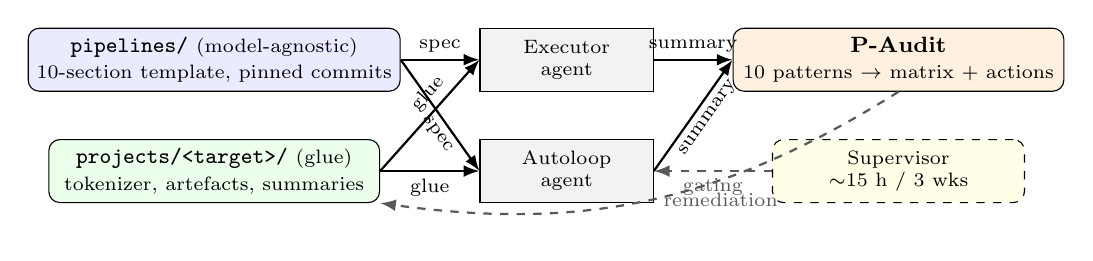
\begin{tikzpicture}[
  font=\footnotesize,
  node distance=6mm and 10mm,
  spec/.style={draw,rounded corners,fill=blue!8,inner sep=3pt,minimum width=42mm,minimum height=8mm,align=center},
  proj/.style={draw,rounded corners,fill=green!8,inner sep=3pt,minimum width=42mm,minimum height=8mm,align=center},
  audit/.style={draw,rounded corners,fill=orange!12,inner sep=3pt,minimum width=42mm,minimum height=8mm,align=center},
  agent/.style={draw,fill=gray!10,inner sep=2pt,minimum width=22mm,minimum height=8mm,align=center,font=\scriptsize},
  sup/.style={draw,dashed,rounded corners,fill=yellow!10,inner sep=2pt,minimum width=32mm,minimum height=8mm,align=center,font=\scriptsize},
  arr/.style={-{Latex[length=2mm]},thick},
  arrd/.style={-{Latex[length=2mm]},thick,dashed,gray!70!black}
]
\node[spec] (pipes) {\texttt{pipelines/} \scriptsize (model-agnostic)\\ \scriptsize 10-section template, pinned commits};
\node[proj,below=of pipes] (proj) {\texttt{projects/<target>/} \scriptsize (glue)\\ \scriptsize tokenizer, artefacts, summaries};
\node[agent,right=of pipes] (a1) {Executor\\agent};
\node[agent,below=of a1] (a2) {Autoloop\\agent};
\node[audit,right=of a1] (audit) {\textbf{P-Audit}\\ \scriptsize 10 patterns $\to$ matrix + actions};
\node[sup,below=of audit] (sup) {Supervisor\\ \scriptsize $\sim$15 h / 3 wks};

\draw[arr] (pipes) -- node[above=-1pt,font=\scriptsize]{spec} (a1);
\draw[arr] (pipes.east) -- node[pos=0.6,sloped,below=-1pt,font=\scriptsize]{spec} (a2.west);
\draw[arr] (proj.east) -- node[pos=0.6,sloped,above=-1pt,font=\scriptsize]{glue} (a1.west);
\draw[arr] (proj) -- node[below=-1pt,font=\scriptsize]{glue} (a2);
\draw[arr] (a1) -- node[above=-1pt,font=\scriptsize]{summary} (audit);
\draw[arr] (a2.east) -- node[pos=0.55,sloped,below=-1pt,font=\scriptsize]{summary} (audit.west);
\draw[arrd] (sup.west) -- node[below=-1pt,font=\scriptsize]{gating} (a2.east);
\draw[arrd] (audit.south) to[bend left=20] node[pos=0.5,right=1pt,font=\scriptsize]{remediation} (proj.south east);
\end{tikzpicture}
\caption{The agent-driven pipeline architecture. Markdown
specifications under \texttt{pipelines/} act as executable
contracts for Claude agents; per-target-model glue lives under
\texttt{projects/<target>/}; the audit pipeline runs after each
batch, applying ten reviewer-derived patterns to produced
artefacts and emitting an action-proposal table. The supervisor
issues run requests, sets chance-baseline expectations, and gates
expensive operations.}
\label{fig:architecture}
\end{figure*}

\subsection{Pipelines as executable specifications}
Each method we deploy lives as a single markdown file in
\texttt{pipelines/} following a frozen 10-section template:
overview, source citation with pinned commit hash, inputs, outputs,
dependencies, methodology with numbered steps, code references
into pinned reference implementations, parameters table,
validation signatures, and known pitfalls. The template is
enforced; missing or out-of-order sections are rejected. The
contract is strong enough that any sufficiently capable LLM agent
can execute the pipeline end-to-end without re-reading the source
paper. Because reviewers' recurring objections cluster around
predictable omissions (missing null model, missing trivial
baseline, missing positive control, missing scope qualifier), each
gets a named slot with non-empty content; an agent that follows
the template inherits much of the methodological hygiene by
construction.

\subsection{Per-target-model project structure}
For each \scfm{}, a directory under \texttt{projects/<target>/}
holds tokenizer wiring, weight-download instructions, run
artefacts, and per-pipeline summaries. Pipelines are
model-agnostic; the project directory holds the model-specific
glue. The split lets the same catalogue deploy against multiple
\scfm{}s without modifying the pipelines, and lets new pipelines
be added against an existing \scfm{} without re-extracting
embeddings.

\subsection{Coordination and supervision}
Most pipelines are single-agent. For pipelines with open-ended
hypothesis search (the topology-141 pipeline, the
manifold-discovery sweep), an autonomous loop alternates
``brainstormer'' and ``executor'' turns; we adopt a
\textbf{2-consecutive-negatives retirement rule} to prevent the
loop from re-testing variants of an exhausted hypothesis.
Persistent file-based memory across conversations is essential for
multi-day runs. The supervisor issues run requests, specifies
chance-baseline expectations before launch, and gates expensive
operations, but does not write extraction code, debug runs, or
compose summaries. Across the full \maxtoki{} project, human
supervision totalled $\sim$15 hours over three weeks against
$\sim$50 GPU-hours of agent compute.

\subsection{The recurring-issue audit pipeline}
\label{sec:audit}

We extracted ten recurring methodological objections from six
independent peer-reviewer comment sets in the authors' prior work
and codified them as a reusable checklist (Table~\ref{tab:audit}).
Each pattern has a diagnostic signature, a prescription, and a
citation back to the review documents that established the
pattern. The audit runs end-to-end on a project folder in 1--2
days of agent time and produces a per-pattern $8 \times 10$
verdict matrix and an action-proposal table. The audit itself
is executed autonomously by an agent against artefacts produced by
prior agent runs, so its validity rests on the checklist being
more reliable than any individual run --- an assumption we
revisit in \S\ref{sec:discussion}. The audit has been validated
only on this project; transfer to held-out research projects
remains open.

\begin{table}[t]
\centering
\small
\caption{The 10-pattern audit checklist. P1--P10 codify recurring
peer-reviewer objections from six independent reviews of papers in
the authors' prior work.}
\label{tab:audit}
\begin{tabular}{ll}
\toprule
\textbf{Pattern} & \textbf{Description} \\
\midrule
P1 & Weak null / not anchored to chance \\
P2 & Trivial / gene-level baseline absent \\
P3 & Endpoint--object mismatch \\
P4 & Pseudoreplication / leaky CV \\
P5 & Selection-driven inflation \\
P6 & No positive control for null findings \\
P7 & Single-condition generalization \\
P8 & Stability of headline numbers \\
P9 & Causal language overreach \\
P10 & Reproducibility scaffolding \\
\bottomrule
\end{tabular}
\end{table}

\section{Application: \maxtoki{}}

\subsection{Why \maxtoki{}}

\maxtoki{} was selected as the application target for three
reasons. (1)~\emph{Frontier model.} It is the most recent major
\scfm{} release at the time of writing (March~2026), from the
Theodoris/NVIDIA team, scaling pre-training to $\sim$1T gene tokens
across $\sim$175M human single-cell transcriptomes spanning birth
through 90+~years~\citep{maxtoki2026}. (2)~\emph{New data and
training regime.} Unlike scGPT (encoder-only, rank-binned values)
or Geneformer (encoder-only, rank-ordered Ensembl IDs), \maxtoki{}
is an autoregressive Llama-architecture transformer trained in
two stages, generation followed by trajectory modelling. Context
length is therefore a \emph{trajectory-length} budget --- a cell
occupies one position --- not a per-cell gene-count budget; this
breaks the inherited Geneformer convention of $\le 2{,}048$ genes
per cell, and tests whether pipelines built on encoder-only
\scfm{}s port to the autoregressive trajectory regime. (3)~\emph{An
external port for our catalogue.} The eight pipelines were
developed against scGPT and Geneformer; \maxtoki{} is the first
target outside that family and serves as a stress-test for the
``model-agnostic specification'' claim. Crucially, \maxtoki{}
shares its 20{,}275-token Ensembl-ID gene tokenizer exactly with
\geneformer{}, which makes within-family cross-model alignment
methodologically clean while exposing a cross-architectural-family
scope qualifier (Section~\ref{sec:cross_model}).

\subsection{Target architecture}

\maxtoki{} is a Llama-architecture autoregressive transformer
(11~layers, hidden size 1232, 8~attention heads/layer, vocabulary
20{,}275, context 4{,}096 tokens). The original paper's analyses
focus on cell-state trajectory prediction and steering; ours target
the model's internal representations directly via attention,
residual-stream, and SAE-feature probes.

\subsection{Pipelines deployed}

We deploy eight pipelines against \maxtoki{}
(Table~\ref{tab:pipelines}). The project-specific glue
(gene-symbol-to-token mapping, hidden-state extraction harness,
dataset paths) lives under \texttt{projects/maxtoki/setup/}.

\begin{table}[t]
\centering
\small
\caption{Mech-interp pipelines deployed against \maxtoki{}. Wall
clock is agent-side end-to-end; \mbox{``+ ext.''} denotes
hypothesis-extension phases beyond the base pipeline.}
\label{tab:pipelines}
\begin{tabular}{@{}llr@{}}
\toprule
Pipeline & Probes & Hr. \\
\midrule
\texttt{spectral-geometry} & residual SVD geom. & 0.5 \\
\texttt{attention-grn} ($\times$4) & attention$\to$GRN & 5.5 \\
\texttt{topology-141} & 141-hyp.\ topology & 4+ \\
\texttt{sae-atlas} & TopK SAEs $\sim$5K/L & 2.5 \\
\texttt{sae-circuit-tracing} & 2.1M-edge circuit & 4 \\
\texttt{sae-exhaustive-map.} & 4.97M edges + steer & 5.5+ \\
\texttt{manifold-discovery} & H65 hematopoietic & 24 \\
\texttt{longevity-mechint.} & donor-aware aging & 1.5 \\
\bottomrule
\end{tabular}
\end{table}

\section{Findings}
\label{sec:findings}

A unifying picture emerges: \maxtoki{} encodes cell \emph{identity
geometry} that is recoverable, externally generalizable, and
locally compressible, but encodes fine-grained \emph{regulatory
mechanism} only weakly. The convergent regulatory-logic negative
(\S\ref{sec:convergent_negative}), the manifold positive
(\S\ref{sec:manifold}), and the GATA1 audit-driven re-test
(\S\ref{sec:gata1_inversion}) triangulate this distinction.

\subsection{Convergent negative on regulatory logic}
\label{sec:convergent_negative}

Five methodologically distinct probes agree that \maxtoki{} does
not encode fine-grained TF$\to$target regulatory logic at a
resolution useful for in-silico perturbation. The convergence is
itself the only positive control available for a negative finding:
no single methodological flaw plausibly pushes all five in the same
direction. We note shared assumptions across the probes (model
forward passes, Ensembl-ID tokenizer, partly overlapping
ground-truth databases) and return to common-mode failure modes in
\S\ref{sec:discussion}.

\begin{itemize}[leftmargin=*,itemsep=0pt]
\item \textbf{attention$\to$GRN}: Curveball degree-preserving null
$z\approx 0$ across four runs (K562, RPE1, Adamson,
\maxtokibig{})~\citep{replogle2022perturbseq}; a 1-feature
gene-variance baseline beats attention by 6--20 AUROC points
($p_{\text{BH}}\le 10^{-4}$); residualized AUROC collapses to
chance.
\item \textbf{circuit-tracing} CRISPRi validation: directional
accuracy 53.48\% overall ($n{=}1{,}503{,}408$); per-source mean
53.42\% (95\% CI [52.60\%, 54.16\%]) under
GroupKFold-by-source-gene 5-fold. Real but small.
\item \textbf{sae-atlas} causal-patching specificity: median
$1.01\times$ (paper Geneformer: $2.36\times$); 0/48 TFs
``specific'' under TRRUST --- but see
\S\ref{sec:gata1_inversion}.
\item \textbf{topology-141} signed motif-community (H123):
0--1/12 layers with positive null gap per domain; under strict
dual-axis disjoint CV, immune AUROC drops 0.505$\to$0.462.
\item \textbf{exhaustive-mapping} combinatorial ablation: zero
higher-order synergy (0/2980 superadditive triplets); three-way
redundancy ratio 0.190 (paper: 0.59).
\end{itemize}

\subsection{Manifold discovery as a deployable positive}
\label{sec:manifold}

\maxtoki{}'s residual stream is a multi-axis biological hub. A
7.7~KB hard-sparse operator (16~features $\times$ 60~genes)
extracts a hematopoietic developmental ordering (H65) that passes
four pre-registered quality gates: trustworthiness 0.811 (paired
within-branch shuffle null 0.799); branch-holdout Spearman 0.370
(null $-0.001$); donor-holdout 0.013; permutation $-0.016$. The
branch-holdout gap (0.370 vs.~$-0.001$) is the discriminating
signal. On 13 disjoint donors, trustworthiness is 0.896 (95\%~CI
[0.884, 0.899]); zero-shot transfer to 12 multi-tissue donors
yields 0.827. A non-hematopoietic lung negative control fails 3 of
4 gates decisively. Compactification reduces a 154-dim full-drift
operator to the 7.7~KB sparse form ($2{,}400\times$ compression)
at no quality loss. A sweep over 12 candidate biological rulers
finds two further externally-transferring manifolds (H95 effector
modality, H103 B-cell maturation) plus one
internally-passing (H38 signalling, external transfer not
tested).

The mechanistic substrate is \emph{distributed}: top-4 SVD factors
of the L10H6 head explain only 18.3\% of pooled ablation impact
(paper scGPT: 66.2\%); a top-4 core-sufficiency test collapses
branch from 0.973 to 0.123. The geometry is real and externally
generalizable but does not concentrate in a compact mechanistic
core.

\subsection{Audit-driven re-test of TF specificity}
\label{sec:gata1_inversion}

The \texttt{sae-atlas} TF-specificity test originally reported
0/48 specific under TRRUST: a TF is specific if at least one
significantly-responding SAE feature has $\geq 2$ of its top-20
genes in the TF's TRRUST target set. Audit pattern P6 (no positive
control) flagged this as underpowered: GATA1 has only 57 TRRUST
targets and TAL1 has 10, making the threshold near-impossible
under random feature draws. Re-running the test with feature IDs
retained and evaluating against dorothea ChIP-seq direct
targets~\citep{garcia-alonso2019dorothea} at thresholds
$\{2,3,4,5\}$-of-top-20 (Figure~\ref{fig:gata1}), GATA1's
responding feature 2610 has 8 of its top-20 genes overlapping the
470-element ChIP-seq direct-target set, with $p_{\text{null}} =
0.030$ over 1{,}000 random-feature
draws~\citep{phipson2010permp}.

\begin{figure}[t]
\centering
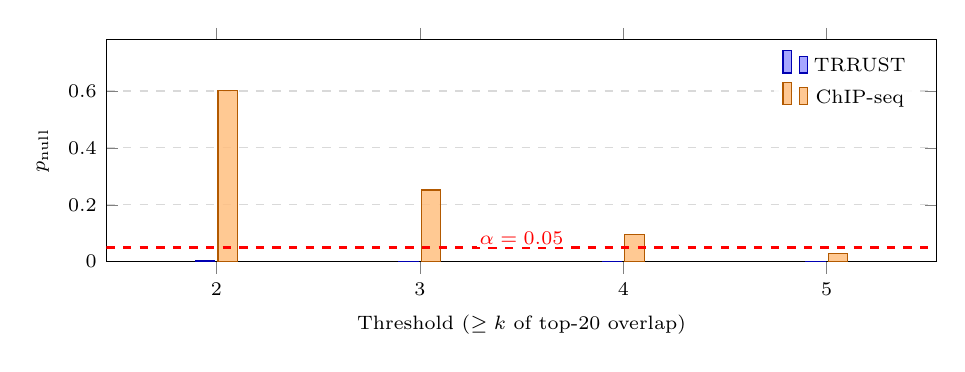
\begin{tikzpicture}
\begin{axis}[
  width=\columnwidth,
  height=4.4cm,
  ybar=1.2pt,
  bar width=7pt,
  ymin=0,ymax=0.78,
  ylabel={$p_{\text{null}}$},
  xlabel={Threshold ($\geq k$ of top-20 overlap)},
  symbolic x coords={2,3,4,5},
  xtick=data,
  enlarge x limits=0.18,
  ymajorgrids=true,grid style={dashed,gray!30},
  legend style={at={(0.98,0.98)},anchor=north east,font=\scriptsize,draw=none,fill=white,fill opacity=0.9,text opacity=1},
  tick label style={font=\scriptsize},
  label style={font=\scriptsize},
  every axis plot/.append style={fill opacity=0.85},
]
\addplot[draw=blue!70!black,fill=blue!40] coordinates {(2,0.003) (3,0.001) (4,0.001) (5,0.001)};
\addplot[draw=orange!70!black,fill=orange!50] coordinates {(2,0.602) (3,0.252) (4,0.096) (5,0.030)};
\draw[red,dashed,thick] ({rel axis cs:0,0}|-{axis cs:2,0.05}) -- ({rel axis cs:1,0}|-{axis cs:2,0.05});
\node[font=\scriptsize,red,fill=white,inner sep=1pt] at ({rel axis cs:0.5,0}|-{axis cs:2,0.05}) [above] {$\alpha=0.05$};
\legend{TRRUST,ChIP-seq}
\end{axis}
\end{tikzpicture}
\caption{GATA1 feature-specificity $p_{\text{null}}$ under TRRUST
(narrow ground truth, 57 targets) vs.~dorothea ChIP-seq direct
targets (470 targets) across thresholds. TRRUST is
near-zero by construction (the headline ``0/48'' was
underpowered); ChIP-seq at strict $\geq 5$ threshold yields
$p_{\text{null}}=0.030$ for $n{=}1$ TF. The threshold was selected
post-hoc; under Bonferroni across the four thresholds
($\alpha/4{=}0.0125$) the result is no longer significant.
Replication on additional cell lines and TFs is required.}
\label{fig:gata1}
\end{figure}

\textbf{Caveats.} The result rests on a single TF (GATA1), in a
single cell line (Replogle K562~\citep{replogle2022perturbseq}),
against a single ChIP-seq dataset, with the threshold selected
post-hoc. MYC and TAL1 are not perturbed in K562 and could not be
tested. The right reading is narrow: the original 0\% verdict is
substantially an artefact of TRRUST narrowness, and under proper
ChIP-seq ground truth there is at most suggestive evidence
($p=0.030$ uncorrected) that \maxtoki{}'s SAE features encode
TF-target regulatory information --- subject to replication.

\subsection{Trajectory steering and cell-state control}
\label{sec:trajectory_steering}

The exhaustive-mapping pipeline's trajectory-steering experiment
provides the project's first \emph{causal positive}: activation
addition along selected SAE features in early-pseudotime Tabula
Sapiens immune cells~\citep{tabulasapiens2022} pushes cell-state
logits toward maturity. Using the spec-compliant
$\Delta s = \cos(z', g_{\text{late}}) - \cos(z', g_{\text{early}})
- \text{baseline}$ metric, $\Delta s$ is positive at L0/L3/L9/L11
and inverts to a counter-differentiation basin at L6
(Figure~\ref{fig:steering}). Top-upregulated genes are
biologically coherent: L0 upregulates SOD3 and KITLG (progenitor /
stemness markers), L6 upregulates C1QB (myeloid complement), L11
upregulates FTL (terminal erythroid ferritin).

\begin{figure}[t]
\centering
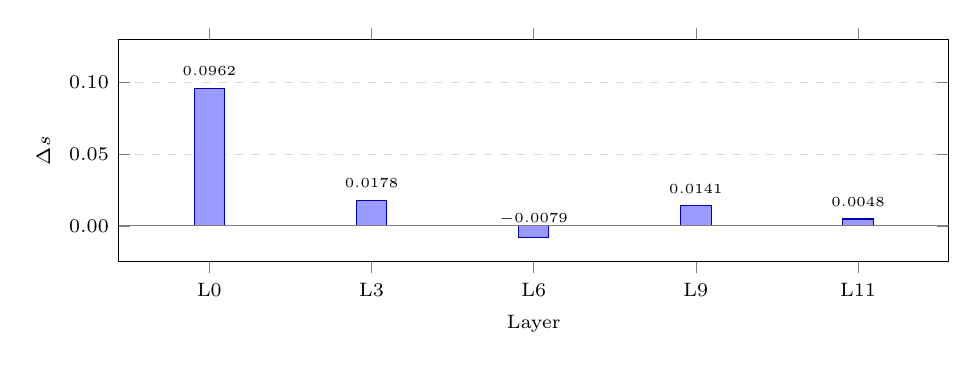
\begin{tikzpicture}
\begin{axis}[
  width=\columnwidth,
  height=4.4cm,
  ybar,
  bar width=11pt,
  ymin=-0.025,ymax=0.13,
  ylabel={$\Delta s$},
  xlabel={Layer},
  symbolic x coords={L0,L3,L6,L9,L11},
  xtick=data,
  enlarge x limits=0.14,
  ymajorgrids=true,grid style={dashed,gray!30},
  tick label style={font=\scriptsize},
  label style={font=\scriptsize},
  yticklabel style={/pgf/number format/.cd,fixed,precision=2,zerofill},
  scaled y ticks=false,
  nodes near coords={\pgfmathprintnumber[fixed,precision=4,zerofill]{\pgfplotspointmeta}},
  nodes near coords style={font=\tiny,anchor=south,yshift=1pt},
  point meta=explicit symbolic,
]
\addplot[draw=blue!70!black,fill=blue!40,nodes near coords align={anchor=south}] coordinates {(L0,0.0962) [+0.0962] (L3,0.0178) [+0.0178] (L6,-0.0079) [-0.0079] (L9,0.0141) [+0.0141] (L11,0.0048) [+0.0048]};
\draw[gray,thin] ({rel axis cs:0,0}|-{axis cs:L0,0}) -- ({rel axis cs:1,0}|-{axis cs:L11,0});
\end{axis}
\end{tikzpicture}
\caption{Activation-steering effect $\Delta s$ across \maxtoki{}
layers. L0 has the largest push toward maturity ($\sim$$20\times$
larger than L11); L6 inverts to counter-differentiation. L9 and
L11 are positive but small; we report them as suggestive (no
permutation null over feature selection was bounded). Unlike
Geneformer's monotone L0$\to$L17
progression~\citep{anon2026exhaustive}, \maxtoki{} shows a
non-monotonic mid-layer basin --- consistent with trajectory-aware
pre-training distributing pseudotemporal information throughout
the stack.}
\label{fig:steering}
\end{figure}

The L0 effect ($\sim$$20\times$ larger than L11) is the clearest
positive; the L9 and L11 magnitudes are near a noise floor for
which we have not bounded a separate permutation null over feature
selection, and are reported as suggestive. The finding is
consistent with the regulatory-logic negative
(\S\ref{sec:convergent_negative}): \maxtoki{} represents cell
\emph{identity} along a differentiation axis, not the
\emph{regulatory mechanism} that moves a cell along it.

\subsection{Cross-architectural scope and cross-layer stability}
\label{sec:cross_model}
\label{sec:cross_layer}

Cross-model alignment with \geneformer{} replicates strongly: CCA
$r{=}0.78$, pairwise gene-similarity Pearson $0.382$ (95\%~CI
$[0.380, 0.384]$). Alignment with scGPT breaks: CCA $r{=}0.40$,
pairwise Pearson $\approx 0$ (slightly negative on immune,
$z{=}{-}3.0$), top-1 retrieval 5--8\% (vs.~38--47\% against
\geneformer{}). scGPT differs from \maxtoki{} in both tokenization
and architecture, so the failure isolates to
architectural-family scope.

Within \maxtoki{}, gene-pair geometry is moderately stable across
layers, depending on the feature construction. Cross-layer Pearson
is 0.604--0.678 for the H123 signed motif-community feature and
0.561 for Euclidean distance, but only 0.275 for the
triangle-defect feature. A correlation of $\sim$$0.65$ shares
$\sim$$40\%$ of variance, so the layers do not encode identical
gene-pair geometry --- the framing is ``moderate conservation,''
not ``no change.'' Within-layer stability and within-family
cross-model agreement appear to project the same observation:
\scfm{} input embeddings carry most of the gene-pair geometric
load.

\section{Audit-Detected Failures}
\label{sec:audit_findings}

Two remediation cycles raised the share of fully addressed audit
patterns from 61\% to 75\% across the eight pipelines. Three
audit-detected failures shifted headline numbers materially:
a sign-tracking error in the original directional-accuracy
implementation (mapping to P3, endpoint--object mismatch); a
TF-specificity test reported as 0/48 without anchoring to a chance
baseline that was near-zero by construction (P1/P6); and several
headline numbers reported as point estimates without bootstrap CIs
(P8). Without the audit pass, this paper would have reported
``0/48 TF specificity'' as a clean negative and ``54.61\%
directional accuracy'' as a positive --- one verdict-level
overconfident in each direction. We have not formally validated
that headlines the audit did \emph{not} flag are equally reliable,
a known limit of an agent-policed-by-agent setup
(\S\ref{sec:discussion}).

\section{Discussion}
\label{sec:discussion}

\paragraph{What worked.} The pipeline-as-spec contract held;
agents executed pipelines without re-reading source papers. The
template caught structural omissions. Persistent file-based memory
was essential for multi-day runs. The 2-consecutive-negatives
retirement rule prevented exhausted-hypothesis loops. The audit
detected three load-bearing flaws.

\paragraph{Common-mode risks for the convergent negative.} The
five probes that converge on the regulatory-logic negative are not
strictly independent: they share model forward passes, the
Ensembl-ID tokenizer, partial overlap in ground-truth databases,
and were developed by the same authors. A single shared confound
--- e.g., training data weighted away from perturbation
experiments, or systematic gene-coverage gaps in the ground-truth
resources --- could push several probes the same way. The
convergence is strong evidence within the assumptions the probes
share; it is not evidence \emph{about} those assumptions.

\paragraph{Generalization.} The catalogue ports cleanly between
\scfm{}s sharing the standard \texttt{transformers}
interface; \maxtoki{} is the first port outside the original scGPT
/ Geneformer family. The audit framework is architecture-
independent at the pattern level. Non-\scfm{} biological
foundation models~\citep{lin2023esm2,jumper2021alphafold,nguyen2024evo,dallatorre2024nucleotide}
remain untested; recent SAE work on protein language
models~\citep{simon2025interplm} suggests a plausible path.

\paragraph{Limitations.} The agent system runs the human-authored
catalogue but does not generate novel pipeline architectures. The
audit framework has been validated on a single project. Three
audit categories were not closed: a cell-level robustness
comparison against scVI / Palantir / CellTypist baselines;
longevity probing at AIDA scale; and cross-architectural
replication of the H123 probe on scGPT. The GATA1 ChIP-seq
inversion rests on $n{=}1$ TF in K562 at a post-hoc-selected
threshold ($p{=}0.030$ uncorrected, marginal under Bonferroni);
replication is the next required step. We have not run a
non-agent baseline on the same pipelines, so the methodological
contribution is documented as a deployment study with an audit
case study, not a head-to-head against human or alternative-agent
execution.

\section{Conclusion}

We applied an agent-driven mech-interp architecture to \maxtoki{},
a recently released trajectory-aware single-cell foundation
model. Approximately 15 hours of high-level human supervision
direct $\sim$50 GPU-hours of agent compute through a
methodologically defensible mech-interp pass yielding six
interrelated findings that jointly characterize \maxtoki{} as
encoding cell-identity geometry but not directed regulatory
mechanism. The pipeline catalogue itself originates in prior work;
the contribution here is the agent-execution architecture, the
reusable audit framework, and the deployment study.

\paragraph{Reproducibility.} Run artefacts, audit reports, and
per-pipeline summaries are released at the project repository
(URL withheld for anonymous review). \maxtoki{}, scGPT,
and \geneformer{} weights are taken from public HuggingFace
releases at revisions pinned in \texttt{projects/<target>/setup/}.
Random seeds, dataset versions, software versions, and per-pipeline
hardware (a single A100-80GB for forward passes; CPU for SAE
training and analysis) are recorded in each run's
\texttt{run.log}.

\bibliographystyle{icml2024}
\bibliography{references}

\end{document}
